\documentclass[12pt]{article}
\usepackage{amsmath}
\usepackage{amssymb}
\usepackage{amsthm}
\providecommand{\abs}[1]{\lvert#1\rvert}
\providecommand{\norm}[1]{\lVert#1\rVert}

\newtheorem{thm}{Theorem}
\newtheorem{lemma}[thm]{Lemma}
\newtheorem{fact}[thm]{Fact}
\newtheorem{cor}[thm]{Corollary}
\newtheorem{eg}{Example}
\newtheorem{ex}{Exercise}
\newtheorem{defi}{Definition}
\newtheorem{hw}{Problem}
\newenvironment{sol}
  {\par\vspace{3mm}\noindent{\it Solution}.}
  {\qed}

\usepackage{algorithm,algorithmic,bm,color}
\floatstyle{plain}
\newfloat{myalgo}{tbhp}{mya}

\newenvironment{Algorithm}[2][tbh]
{\begin{myalgo}[#1]\centering\begin{minipage}{#2}\begin{algorithm}[H]}%
{\end{algorithm}\end{minipage}\end{myalgo}}

% Use the postscript times font!
\usepackage{times}
\usepackage{soul}
\usepackage{url}
\usepackage[hidelinks]{hyperref}
\usepackage[utf8]{inputenc}
\usepackage[small]{caption}
\usepackage{graphicx}
\usepackage{amsmath}
\usepackage{booktabs}
\usepackage{algorithm}
\usepackage{algorithmic}\usepackage{amsfonts}
\urlstyle{same}

\makeatletter
\newenvironment{breakablealgorithm}
{% \begin{breakablealgorithm}
	\begin{center}
		\refstepcounter{algorithm}% New algorithm
		\hrule height.8pt depth0pt \kern2pt% \@fs@pre for \@fs@ruled
		\renewcommand{\caption}[2][\relax]{% Make a new \caption
			{\raggedright\textbf{\ALG@name~\thealgorithm} ##2\par}%
			\ifx\relax##1\relax % #1 is \relax
			\addcontentsline{loa}{algorithm}{\protect\numberline{\thealgorithm}##2}%
			\else % #1 is not \relax
			\addcontentsline{loa}{algorithm}{\protect\numberline{\thealgorithm}##1}%
			\fi
			\kern2pt\hrule\kern2pt
		}
	}{% \end{breakablealgorithm}
		\kern2pt\hrule\relax% \@fs@post for \@fs@ruled
	\end{center}
}
\makeatother

\setlength{\parindent}{0pt}
%\setlength{\parskip}{2ex}
\newenvironment{proofof}[1]{\bigskip\noindent{\itshape #1. }}{\hfill$\Box$\medskip}

\usepackage{enumerate,fullpage,proof}

% the following package is optional:
%\usepackage{latexsym} 
\usepackage{amsfonts}
\usepackage{subfigure}
\usepackage{booktabs}
\usepackage{stfloats}
\usepackage{amssymb}
\DeclareMathOperator{\diag}{diag}
\DeclareMathOperator{\mst}{s.t.}
\renewcommand{\algorithmicrequire}{\textbf{Input:}}
\renewcommand{\algorithmicensure}{\textbf{Output:}}

\newcommand{\argmin}{\arg\!\min}
\newcommand{\argmax}{\arg\!\max}
\newcommand{\Amat}{{\boldsymbol A}}
\newcommand{\Bmat}{{\boldsymbol B}}
\newcommand{\Cmat}{{\boldsymbol C}}
\newcommand{\Dmat}{{\boldsymbol D}}
\newcommand{\Emat}[0]{{{\boldsymbol E}}}
\newcommand{\Fmat}[0]{{{\boldsymbol F}}}
\newcommand{\Gmat}[0]{{{\boldsymbol G}}}
\newcommand{\Hmat}[0]{{{\boldsymbol H}}}
\newcommand{\Imat}{{\boldsymbol I}}
\newcommand{\Jmat}[0]{{{\boldsymbol J}}}
\newcommand{\Kmat}[0]{{{\boldsymbol K}}}
\newcommand{\Lmat}[0]{{{\boldsymbol L}}}
\newcommand{\Mmat}[0]{{{\boldsymbol M}}}
\newcommand{\Nmat}[0]{{{\boldsymbol N}}}
\newcommand{\Omat}[0]{{{\boldsymbol O}}}
\newcommand{\Pmat}[0]{{{\boldsymbol P}}}
\newcommand{\Qmat}[0]{{{\boldsymbol Q}}}
\newcommand{\Rmat}[0]{{{\boldsymbol R}}}
\newcommand{\Smat}[0]{{{\boldsymbol S}}}
\newcommand{\Tmat}[0]{{{\boldsymbol T}}}
\newcommand{\Umat}{{{\boldsymbol U}}}
\newcommand{\Vmat}[0]{{{\boldsymbol V}}}
\newcommand{\Wmat}[0]{{{\boldsymbol W}}}
\newcommand{\Xmat}{{\boldsymbol X}}
\newcommand{\Ymat}[0]{{{\boldsymbol Y}}}
\newcommand{\Zmat}{{\boldsymbol Z}}

\newcommand{\av}{\boldsymbol{a}}
\newcommand{\Av}{\boldsymbol{A}}
\newcommand{\Cv}{\boldsymbol{C}}
\newcommand{\bv}{\boldsymbol{b}}
\newcommand{\cv}{{\boldsymbol{c}}}
\newcommand{\dv}{\boldsymbol{d}}
\newcommand{\ev}[0]{{\boldsymbol{e}}}
\newcommand{\fv}{\boldsymbol{f}}
\newcommand{\Fv}[0]{{\boldsymbol{F}}}
\newcommand{\gv}[0]{{\boldsymbol{g}}}
\newcommand{\hv}[0]{{\boldsymbol{h}}}
\newcommand{\iv}[0]{{\boldsymbol{i}}}
\newcommand{\jv}[0]{{\boldsymbol{j}}}
\newcommand{\kv}[0]{{\boldsymbol{k}}}
\newcommand{\lv}[0]{{\boldsymbol{l}}}
\newcommand{\mv}[0]{{\boldsymbol{m}}}
\newcommand{\nv}{\boldsymbol{n}}
\newcommand{\ov}[0]{{\boldsymbol{o}}}
\newcommand{\pv}[0]{{\boldsymbol{p}}}
\newcommand{\qv}[0]{{\boldsymbol{q}}}
\newcommand{\rv}[0]{{\boldsymbol{r}}}
\newcommand{\sv}[0]{{\boldsymbol{s}}}
\newcommand{\tv}[0]{{\boldsymbol{t}}}
\newcommand{\uv}[0]{{\boldsymbol{u}}}
\newcommand{\vv}{\boldsymbol{v}}
\newcommand{\wv}{\boldsymbol{w}}
\newcommand{\Wv}{\boldsymbol{W}}
\newcommand{\xv}{\boldsymbol{x}}
\newcommand{\yv}{\boldsymbol{y}}
\newcommand{\Xv}{\boldsymbol{X}}
\newcommand{\Yv}{\boldsymbol{Y}}
\newcommand{\zv}{\boldsymbol{z}}

\newcommand{\xvf}{\widetilde{\xv}}
\newcommand{\Fmb}{\boldsymbol{\mathcal{F}}}

\newcommand{\Gammamat}[0]{{\boldsymbol{\Gamma}}}
\newcommand{\Deltamat}[0]{{\boldsymbol{\Delta}}}
\newcommand{\Thetamat}{\boldsymbol{\Theta}}
\newcommand{\Lambdamat}{{\boldsymbol{\Lambda}}}
\newcommand{\Ximat}[0]{{\boldsymbol{\Xi}}}
\newcommand{\Pimat}[0]{{\boldsymbol{\Pi}} }
\newcommand{\Sigmamat}{\boldsymbol{\Sigma}}
\newcommand{\Upsilonmat}[0]{{\boldsymbol{\Upsilon}} }
\newcommand{\Phimat}{\boldsymbol{\Phi}}
\newcommand{\Psimat}{\boldsymbol{\Psi}}
\newcommand{\Omegamat}{{\boldsymbol{\Omega}}}

\newcommand{\Lambdav}{\bm{\Lambda}}
\newcommand{\alphav}{\boldsymbol{\alpha}}
\newcommand{\betav}[0]{{\boldsymbol{\beta}} }
\newcommand{\gammav}{{\boldsymbol{\gamma}}}
\newcommand{\deltav}[0]{{\boldsymbol{\delta}} }
\newcommand{\epsilonv}{\boldsymbol{\epsilon}}
\newcommand{\zetav}[0]{{\boldsymbol{\zeta}} }
\newcommand{\etav}[0]{{\boldsymbol{\eta}} }
\newcommand{\thetav}{\boldsymbol{\theta}}
\newcommand{\iotav}[0]{{\boldsymbol{\iota}} }
\newcommand{\kappav}{{\boldsymbol{\kappa}}}
\newcommand{\lambdav}[0]{{\boldsymbol{\lambda}} }
\newcommand{\muv}{\boldsymbol{\mu}}
\newcommand{\nuv}{{\boldsymbol{\nu}}}
\newcommand{\xiv}{{\boldsymbol{\xi}}}
\newcommand{\omicronv}[0]{{\boldsymbol{\omicron}} }
\newcommand{\piv}{\boldsymbol{\pi}}
\newcommand{\rhov}[0]{{\boldsymbol{\rho}} }
\newcommand{\sigmav}[0]{{\boldsymbol{\sigma}} }
\newcommand{\tauv}[0]{{\boldsymbol{\tau}} }
\newcommand{\upsilonv}[0]{{\boldsymbol{\upsilon}} }
\newcommand{\phiv}{\boldsymbol{\phi}}
\newcommand{\chiv}[0]{{\boldsymbol{\chi}} }
\newcommand{\psiv}{\boldsymbol{\psi}}
\newcommand{\omegav}[0]{{\boldsymbol{\omega}} }

\newcommand{\tsp}{^{\mathsf{T}}}
\newcommand{\inv}{^{-1}}
\newcommand{\ie}{{\em i.e.}}
\newcommand{\wrt}{{\em w.r.t.\,}}
\begin{document}

$\;$\hfill Due: 2019/4/14

\begin{center}
{\LARGE\bf Homework 1}
\end{center}


\begin{hw}
K-mean vs GMM (Variant of K-mean).
\begin{sol}
	\begin{enumerate}
		\item[(1)]{
			Derivation	
			
			In this section, I will modify the soft assignment to hard assignment. In another word, I will assign the data point to a specific cluster, which is similar to K-mean method.  
			
			Similar to GMM model, I introduce a latent variable $\zv$ to represent the cluster to which a point $\xv$ belongs, \ie 
			$$\zv = (z_1,\ldots,z_K),$$
			$$z_k\in\{0,1\},~\forall~k\in\{1,\ldots,K\},$$
			$$\sum_{k}^{K}z_k = 1,$$
			$$p(z_k=1) = \pi_k,~0\ge\pi_k\le1,~\sum_{k}^{K}\pi_k = 1,$$
			$$\xv_n = (x_1,\ldots,x_p)^T,~\forall~n\in\{1,\ldots,N\}.$$
			
			I then assume that the points in the same cluster follow the same Gaussian distribution:
			$$p(\xv|z_k=1) = \mathcal{N}(\xv|\muv_k,\Sigmamat_k),$$
			
			I get the distribution for data point $\xv$:
			$$p(\xv) = \sum_{k}^{K}p(\zv)p(\xv|\zv) = \sum_{k}^{K}\pi_k\mathcal{N}(\xv|\muv_k,\Sigmamat_k).$$
		
			I further define the $r_{nk}$, which is similar to the definition in the K-mean algorithm.
			$$
				r_{nk} = \left\{
					\begin{aligned}
					1&~~~,k=\argmax_j~\pi_j\mathcal{N}(\xv_n|\muv_j,\Sigmamat_j)\\
					0&~~~,otherwise.
					\end{aligned}
				\right.
			$$
			
			I call this the E step in our algorithm, since I evaluate the cluster to which the point $\xv_n$ should belong in this step. What's more, with these $r_{nk}$,  $\forall n\in\{1,\ldots,N\}$, I can re-estimate the parameters of the K Gaussian distributions. And this is our M step.
			
			The M step can be described in mathematic way:
			$$N_k = \sum_{n=1}^{N} r_{nk}$$
			$$\muv_k^{new} = \frac{1}{N_k}\sum_{n=1}^{N}r_{nk}\xv_n$$
			$$\Sigmamat_k^{new} = \frac{1}{N_k}\sum_{n=1}^{N}r_{nk}(\xv_n-\muv_k^{new})(\xv_n-\muv_k^{new})^{T}$$
			$$\pi_k^{new} = \frac{N_k}{N}$$
				
		}
		\item[(2)]{
			Algorithm
			
			The algorithm is described in detail with pseudo code in the appendix A.
		}
		\item[(3)]{
			Advantages
			
			Compare our algorithm with GMM, the calculation of ours is reduced since each data point I only consider the most suitable distribution. This is achieved by hard assignment.
			
			When compared with K-mean, our algorithm outperforms K-mean in dealing with the anisotropism inside the data points, because our algorithm utilizes the variance of the data. 
		}
		\item[(4)]{
			Limitations
			
			I did not consider the features of competitive learning in this algorithm. Our algorithm still faces the similar limitations as the GMM and K-mean. The result is influenced by the initialization and it usually is not a global optimization. Though the convergence is guaranteed, it may take a long time to converge. The parameter K still needs to be set manually.
		}
	\end{enumerate}
\end{sol}
\end{hw}

\begin{hw}
K-mean vs CL
\begin{sol}
	\begin{enumerate}
		\item[(1)]{ 
			Derivation
			
			The competitive learning algorithm is similar to K-mean. The different between them is that the CL is an adaptive algorithm and the dataset is a sequence of data coming one by one, while the inputs of K-mean are batches of data.
			
			Thus, I can apply the idea of RPCL into the K-mean. I can modify the definition of $r_{nk}$ as follows:
			$$
				r_{nk} = \left\{
				\begin{aligned}
				1&~~~,k=c,~c = \argmax_j~\pi_j\mathcal{N}(\xv_n|\muv_j,\Sigmamat_j)\\
				-\eta&~~~,k=b,~b=\argmax_{j\ne c}~\pi_j\mathcal{N}(\xv_n|\muv_j,\Sigmamat_j)\\
				0&~~~,otherwise.
				\end{aligned}
				\right.
			$$
			
			For $r_{nk}$ which is equal to 1, I apply the same method to update the $\muv_k$. In another words, I neglect the $r_{nk}$ which is equal to $-\eta$ in the following equation:
			$$\muv_k = \frac{\sum_{n}r_{nk}\xv_n}{\sum_{n}r_{nk}}.$$
			As for $r_{nk}=-\eta$, I apply the thoughts of RPCL. In this way, the rival clusters would move away from the cluster, as the equation
			$$\muv_j = \muv_j + \sum_{k}\sum_{n}r_{nk}(\muv_k-\muv_j)$$
			shows.
			
			But different from the RPCL, the $\eta$ should decrease during the optimization process. If the $\eta$ is a constant, the $\muv$ will continue changing when it should converge. Because the $\eta$ makes the k-th cluster $\muv_k$ away from the its real position even when the rival has been removed far away enough. Thus I consider modify the penalizing parameter to $\eta/t$, where $t$ is the iteration times. As the iteration time increases, the penalizing parameter decreases. 
			
			There's another important point that we should label the deserted clusters in time. Because we update the variance of the distribution of clusters during the iteration. If we don't eliminate the cluster which is moved far away from data in time, the variance of it could become very large when we estimate the Gaussian distribution. This is critical in implementation. 
		}
		\item[(2)]{
			Algorithm
		
			The algorithm is described in detail with pseudo code in the appendix B.
		}
		\item[(3)]{ 
			Implementation
			
			I implemented the algorithm above in Python. Then I test the performance with a dataset consisting three randomly generated clusters. The result is shown in Fig. (\ref{fig_rpkmean}).
			\begin{figure}[ht]
				\centering
				\subfigure[Three cluster with four clusters being initialized.]{
					\begin{minipage}[t]{0.2\linewidth}
						\centering	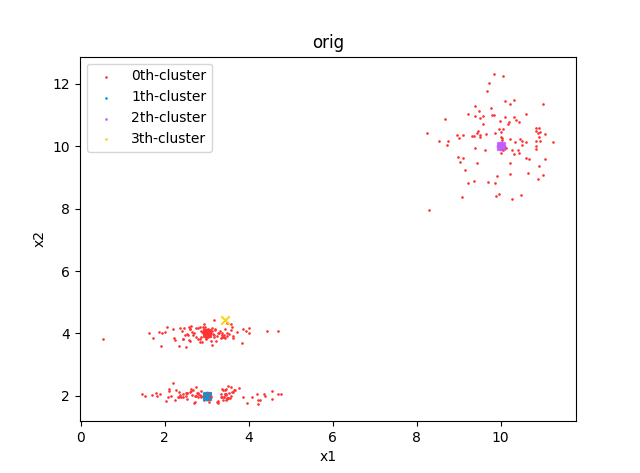
\includegraphics[width=\linewidth, height =3.5cm]{Figs/rp1/1.png}
					\end{minipage}
					\begin{minipage}[t]{0.2\linewidth}
						\centering	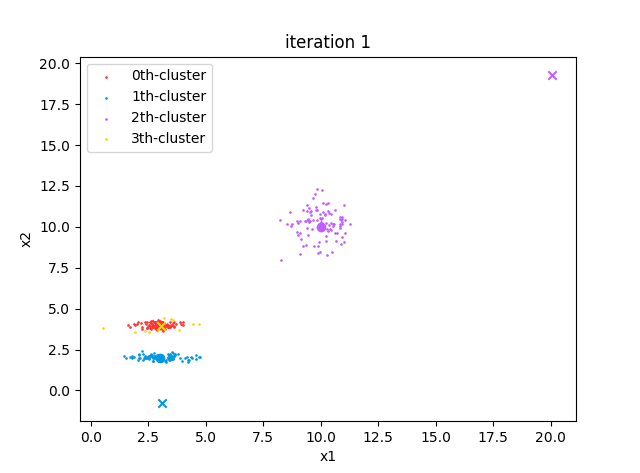
\includegraphics[width=\linewidth, height =3.5cm]{Figs/rp1/2.png}
					\end{minipage}
					\begin{minipage}[t]{0.2\linewidth}
						\centering	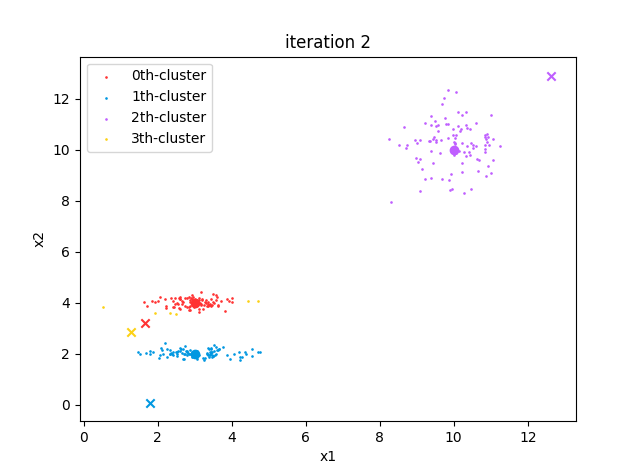
\includegraphics[width=\linewidth, height =3.5cm]{Figs/rp1/3.png}
					\end{minipage}
					\begin{minipage}[t]{0.2\linewidth}
						\centering	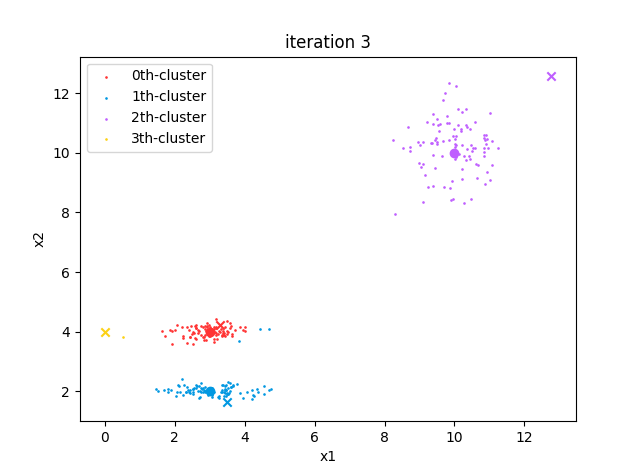
\includegraphics[width=\linewidth, height =3.5cm]{Figs/rp1/4.png}
					\end{minipage}
					\begin{minipage}[t]{0.2\linewidth}
						\centering	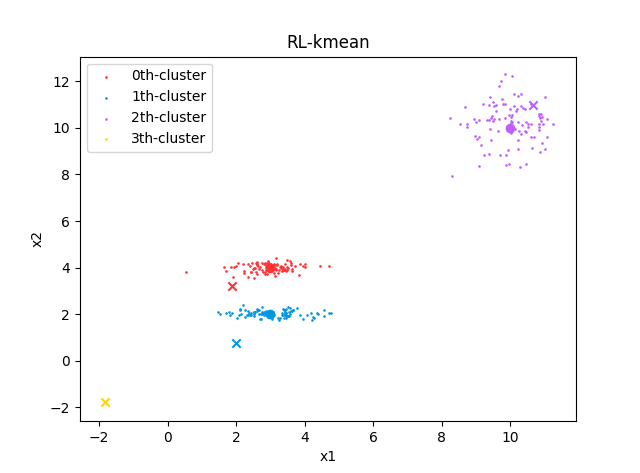
\includegraphics[width=\linewidth, height =3.5cm]{Figs/rp1/5.png}
					\end{minipage}		
				}
				\subfigure[Three cluster with four clusters being initialized.]{
					\begin{minipage}[t]{0.2\linewidth}
						\centering	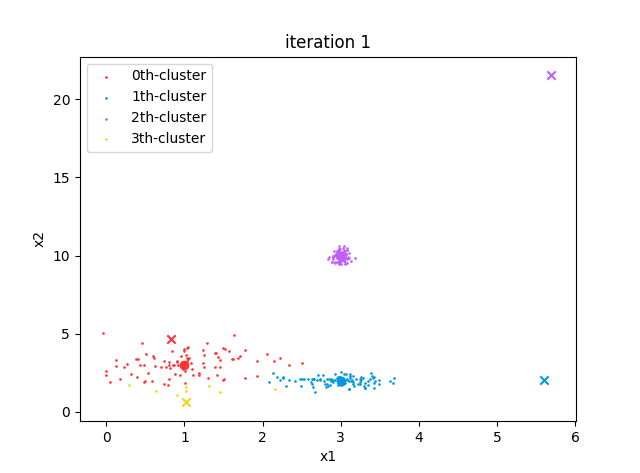
\includegraphics[width=\linewidth, height =3.5cm]{Figs/rp3/1.png}
					\end{minipage}
					\begin{minipage}[t]{0.2\linewidth}
						\centering	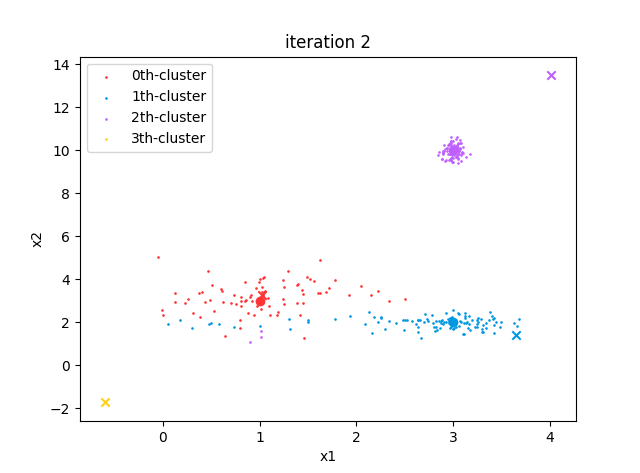
\includegraphics[width=\linewidth, height =3.5cm]{Figs/rp3/2.png}
					\end{minipage}
					\begin{minipage}[t]{0.2\linewidth}
						\centering	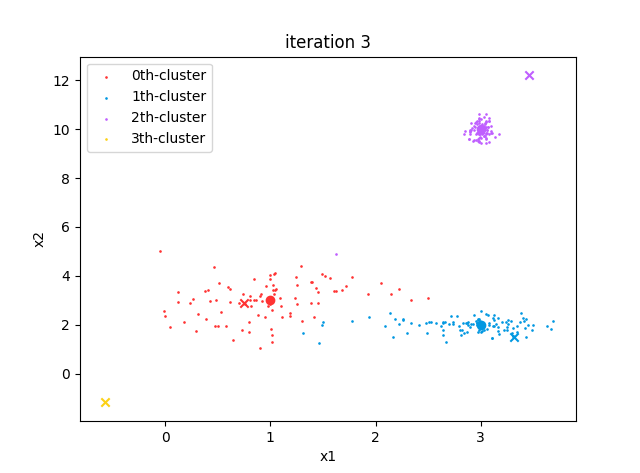
\includegraphics[width=\linewidth, height =3.5cm]{Figs/rp3/3.png}
					\end{minipage}
					\begin{minipage}[t]{0.2\linewidth}
						\centering	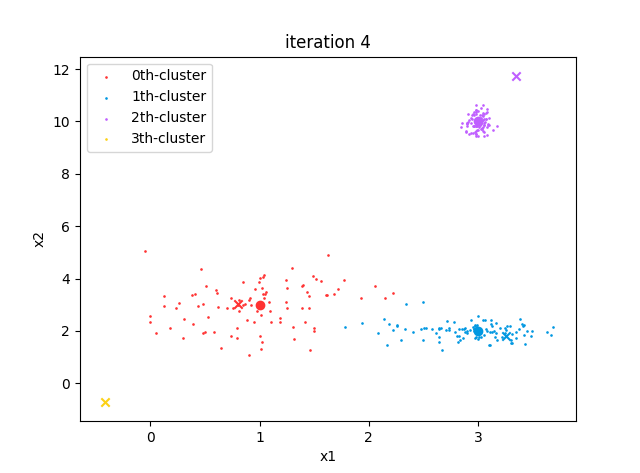
\includegraphics[width=\linewidth, height =3.5cm]{Figs/rp3/4.png}
					\end{minipage}
					\begin{minipage}[t]{0.2\linewidth}
						\centering	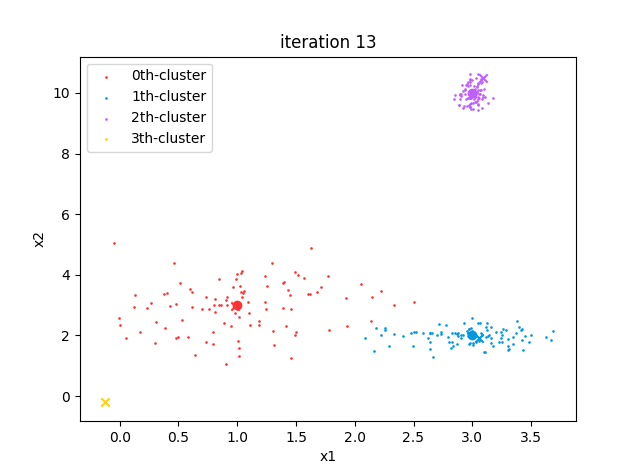
\includegraphics[width=\linewidth, height =3.5cm]{Figs/rp3/5.png}
					\end{minipage}		
				}
				\subfigure[Three cluster with seven clusters being initialized.]{
					\begin{minipage}[t]{0.2\linewidth}
						\centering	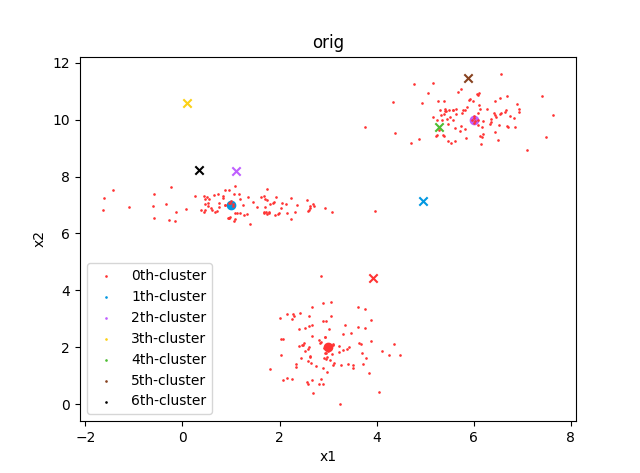
\includegraphics[width=\linewidth, height =3.5cm]{Figs/rp2/1.png}
					\end{minipage}
					\begin{minipage}[t]{0.2\linewidth}
						\centering	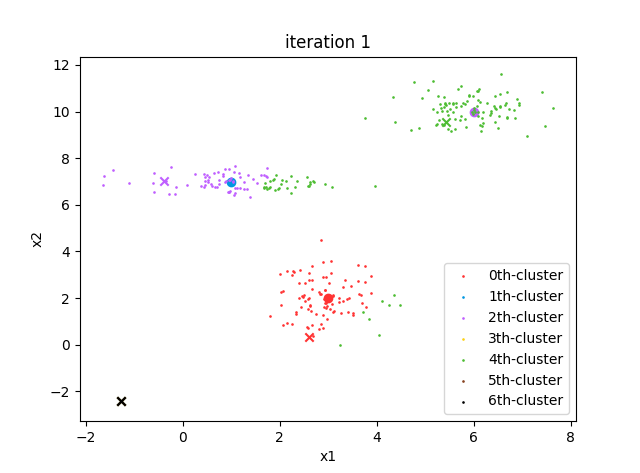
\includegraphics[width=\linewidth, height =3.5cm]{Figs/rp2/2.png}
					\end{minipage}
						\begin{minipage}[t]{0.2\linewidth}
						\centering	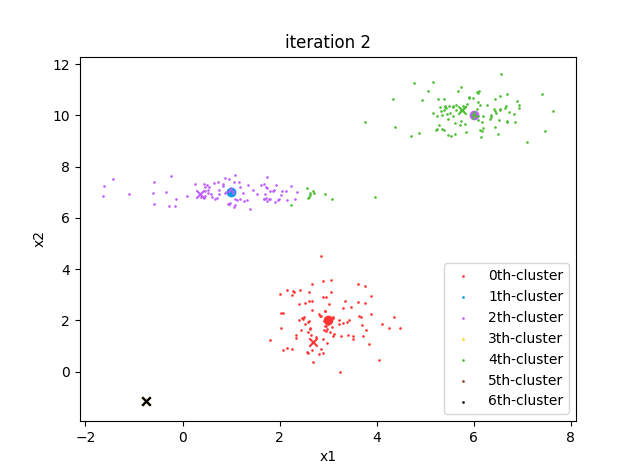
\includegraphics[width=\linewidth, height =3.5cm]{Figs/rp2/3.png}
					\end{minipage}
					\begin{minipage}[t]{0.2\linewidth}
						\centering	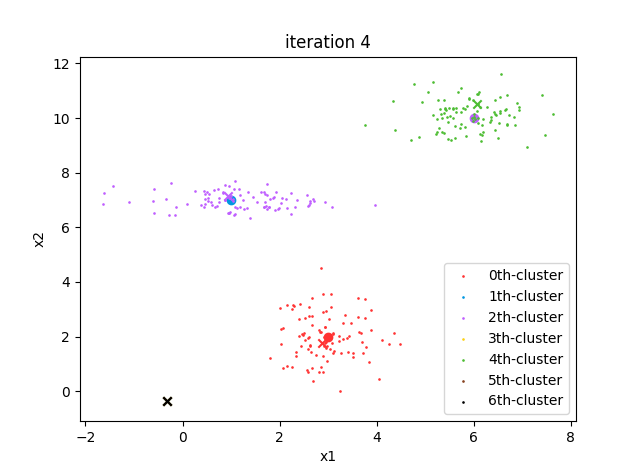
\includegraphics[width=\linewidth, height =3.5cm]{Figs/rp2/4.png}
					\end{minipage}
					\begin{minipage}[t]{0.2\linewidth}
						\centering	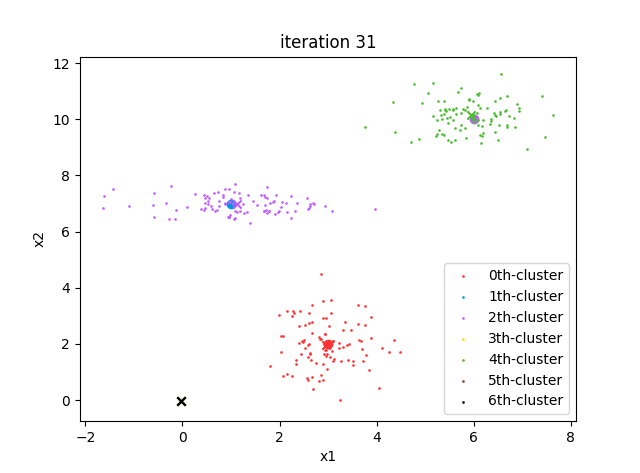
\includegraphics[width=\linewidth, height =3.5cm]{Figs/rp2/5.png}
					\end{minipage}
				}
				\vspace{-4mm}
				\caption{RP K-mean experiments.}
				\label{fig_rpkmean}
				\vspace{-4mm}
			\end{figure}
			
		}
	\end{enumerate}
	
	
\end{sol}	
\end{hw}

\begin{hw}
model selection of GMM
\begin{sol}
	In this section, I used the VBGMM model in sklearn library to do the experiment on VBEM algorithm. The experiment on basic EM algorithm with AIC and BIC criterion is carried twice using the GMM model in sklearn library and the EM algorithm implemented myself. And I will compare the results of them in detail.

	The data is randomly generated from three Gaussian distribution. The initialization of GMM models are also randomly at the beginning. The results are shown in the Fig.~(\ref{fig_GMM_EM}). Compare the GMM model and EM algorithm implemented by myself, and we can find that GMM in scikit-learn library gives a better result than mine. The "dot" is the position of the real means of three clusters, while the "x" is the fitted means of clusters. 

	\begin{figure}[ht]
		\centering
		\subfigure[Three cluster with four clusters being initialized.]{
			\begin{minipage}[t]{0.25\linewidth}
				\centering	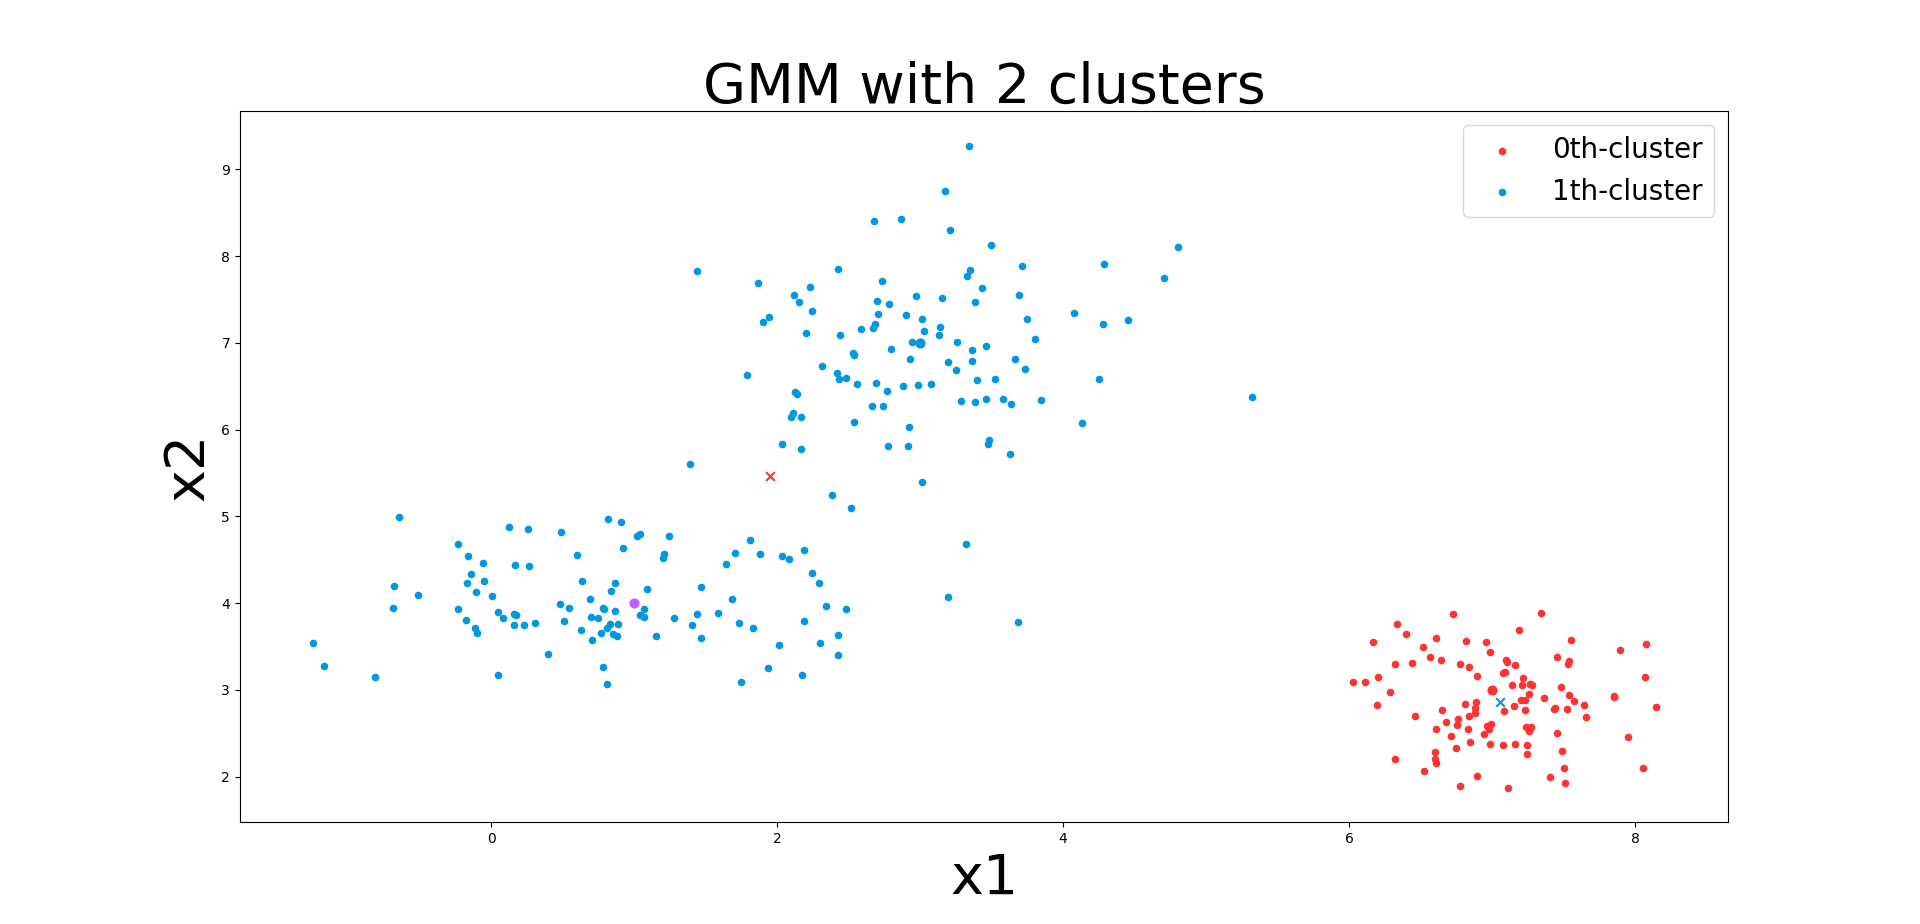
\includegraphics[width=\linewidth, height =3.5cm]{Figs/GMM2.png}
			\end{minipage}
			\begin{minipage}[t]{0.25\linewidth}
				\centering	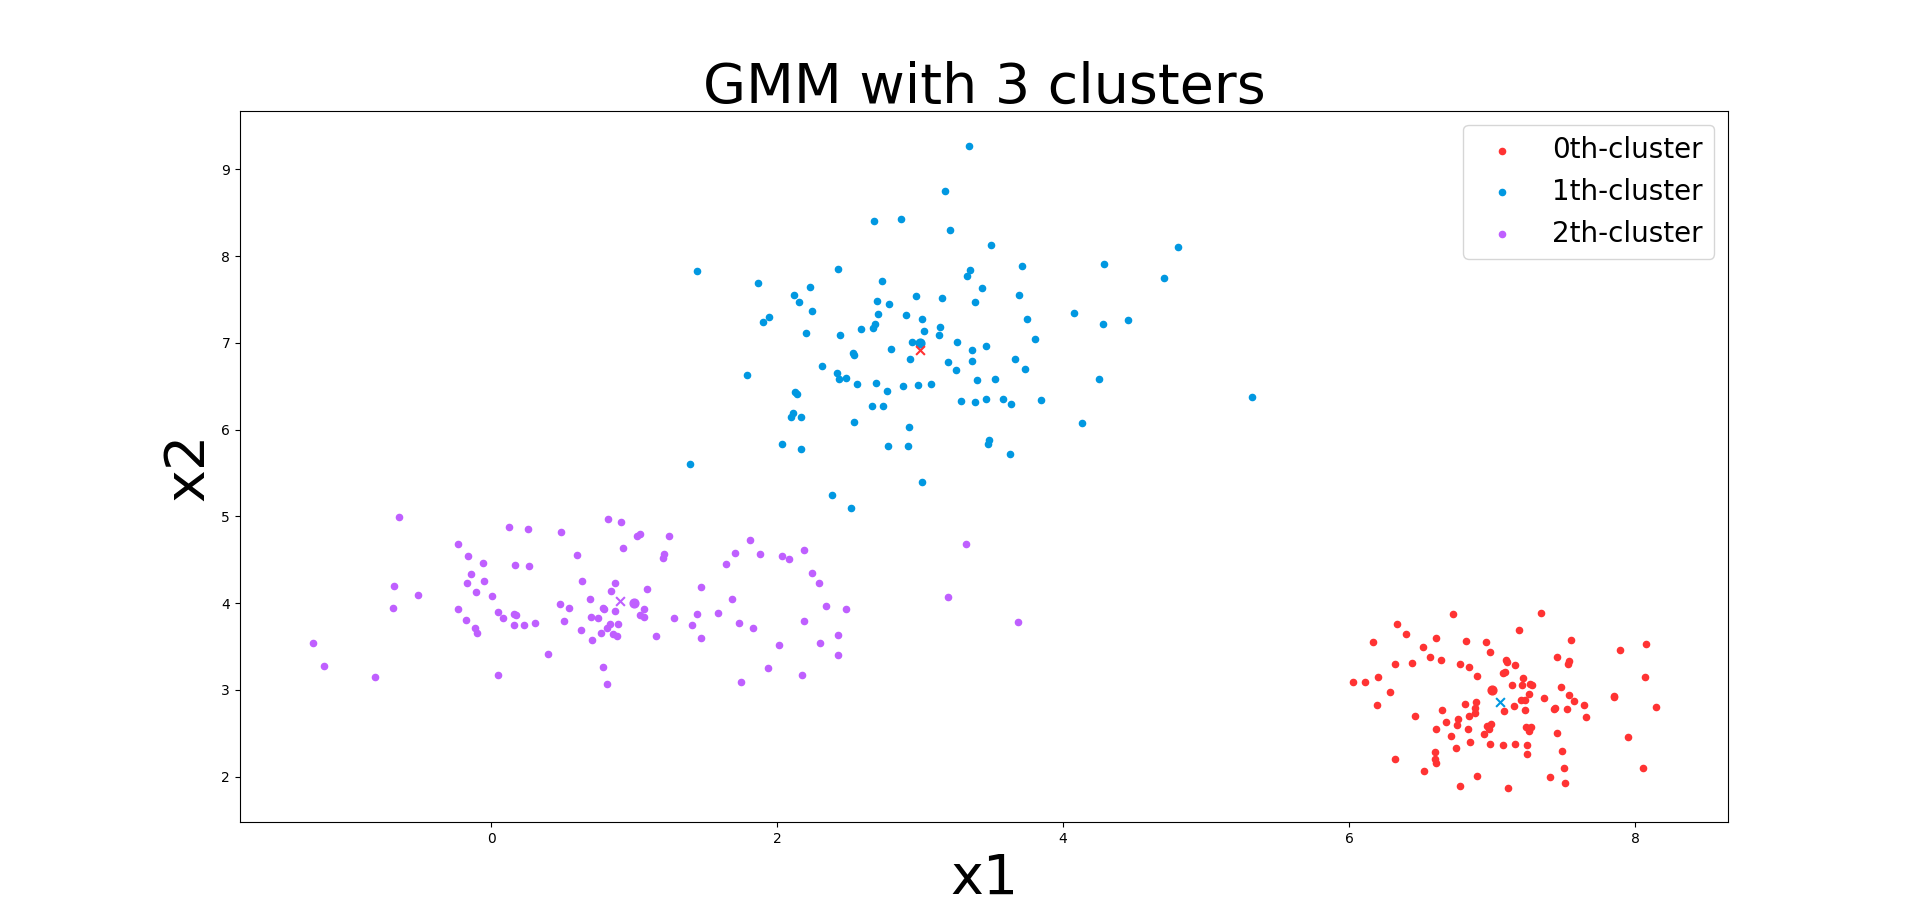
\includegraphics[width=\linewidth, height =3.5cm]{Figs/GMM3.png}
			\end{minipage}
			\begin{minipage}[t]{0.25\linewidth}
				\centering	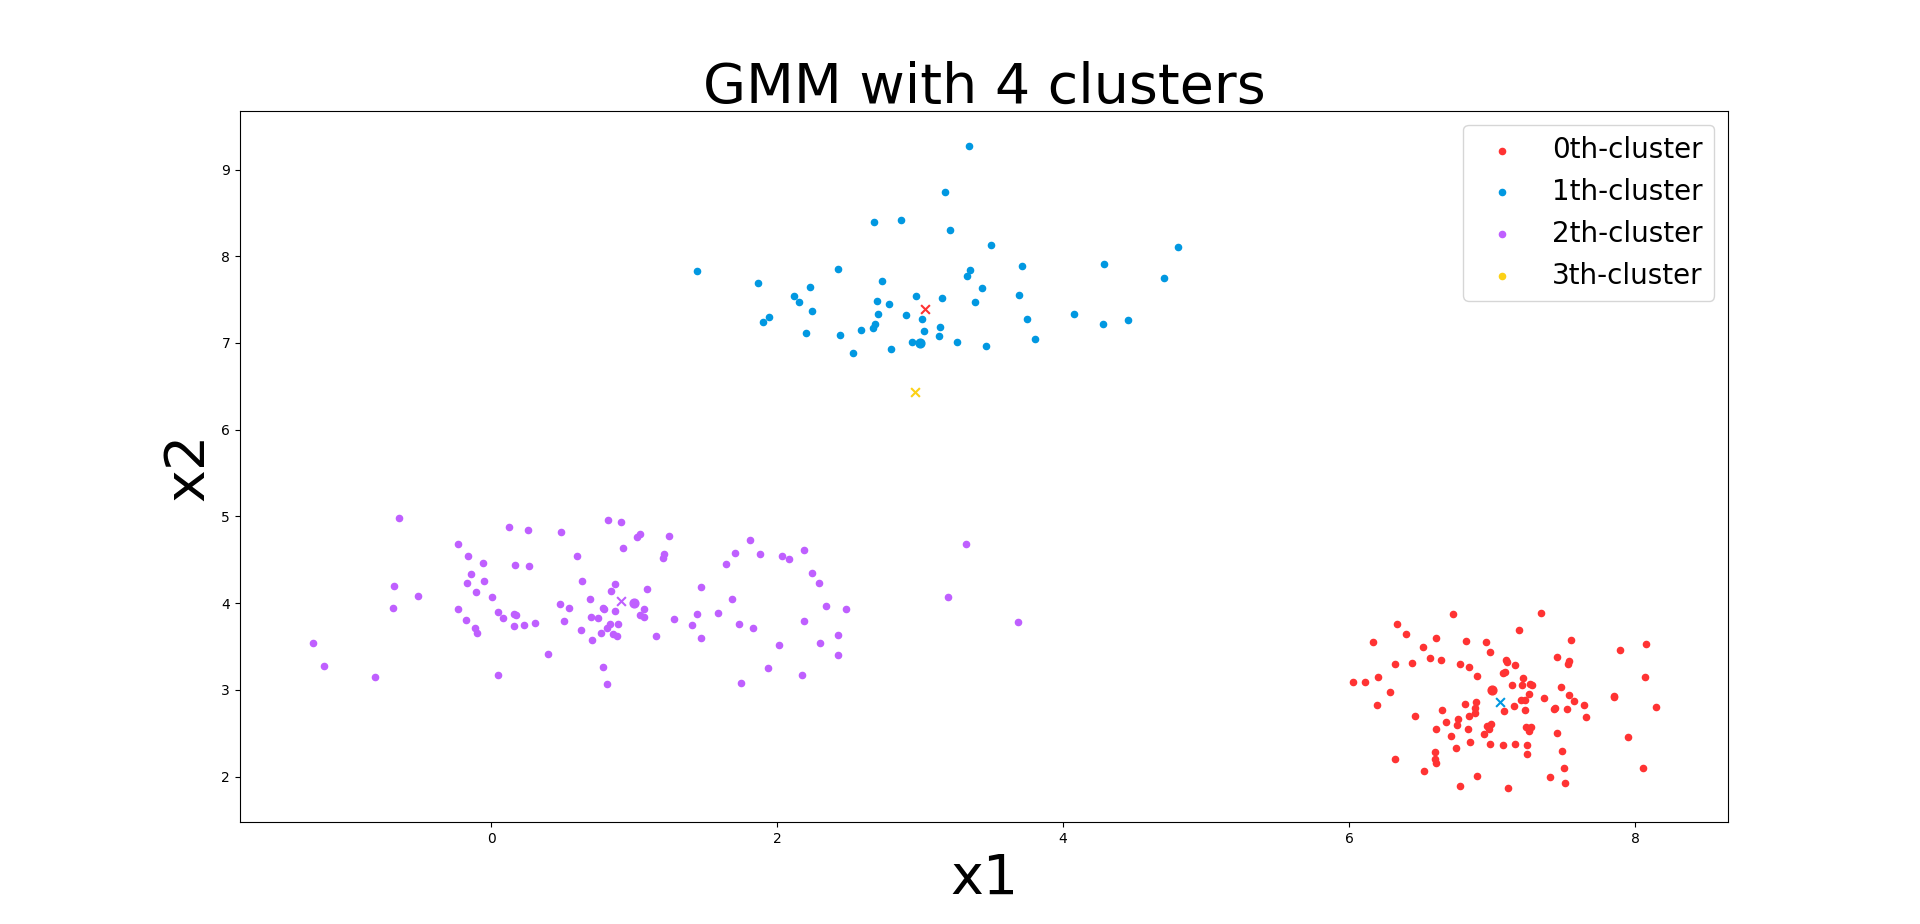
\includegraphics[width=\linewidth, height =3.5cm]{Figs/GMM4.png}
			\end{minipage}
			\begin{minipage}[t]{0.25\linewidth}
				\centering	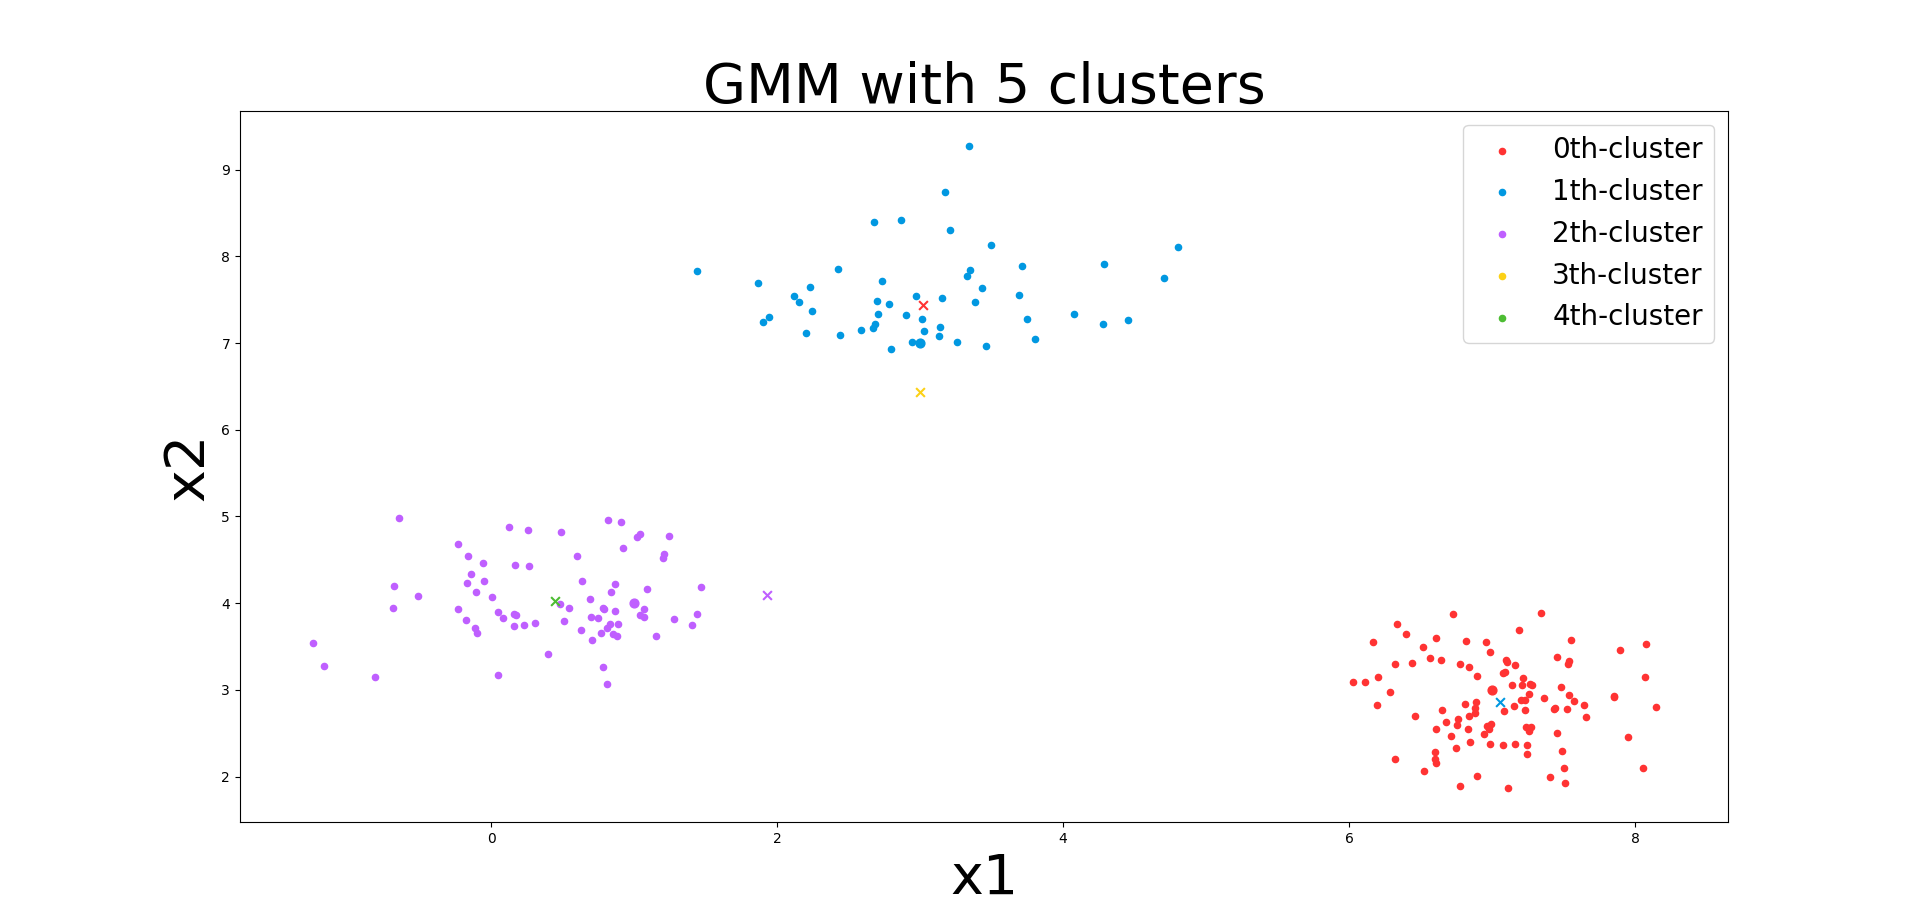
\includegraphics[width=\linewidth, height =3.5cm]{Figs/GMM5.png}
			\end{minipage}	
		}
		\subfigure[Three cluster with seven clusters being initialized.]{
			\begin{minipage}[t]{0.25\linewidth}
				\centering	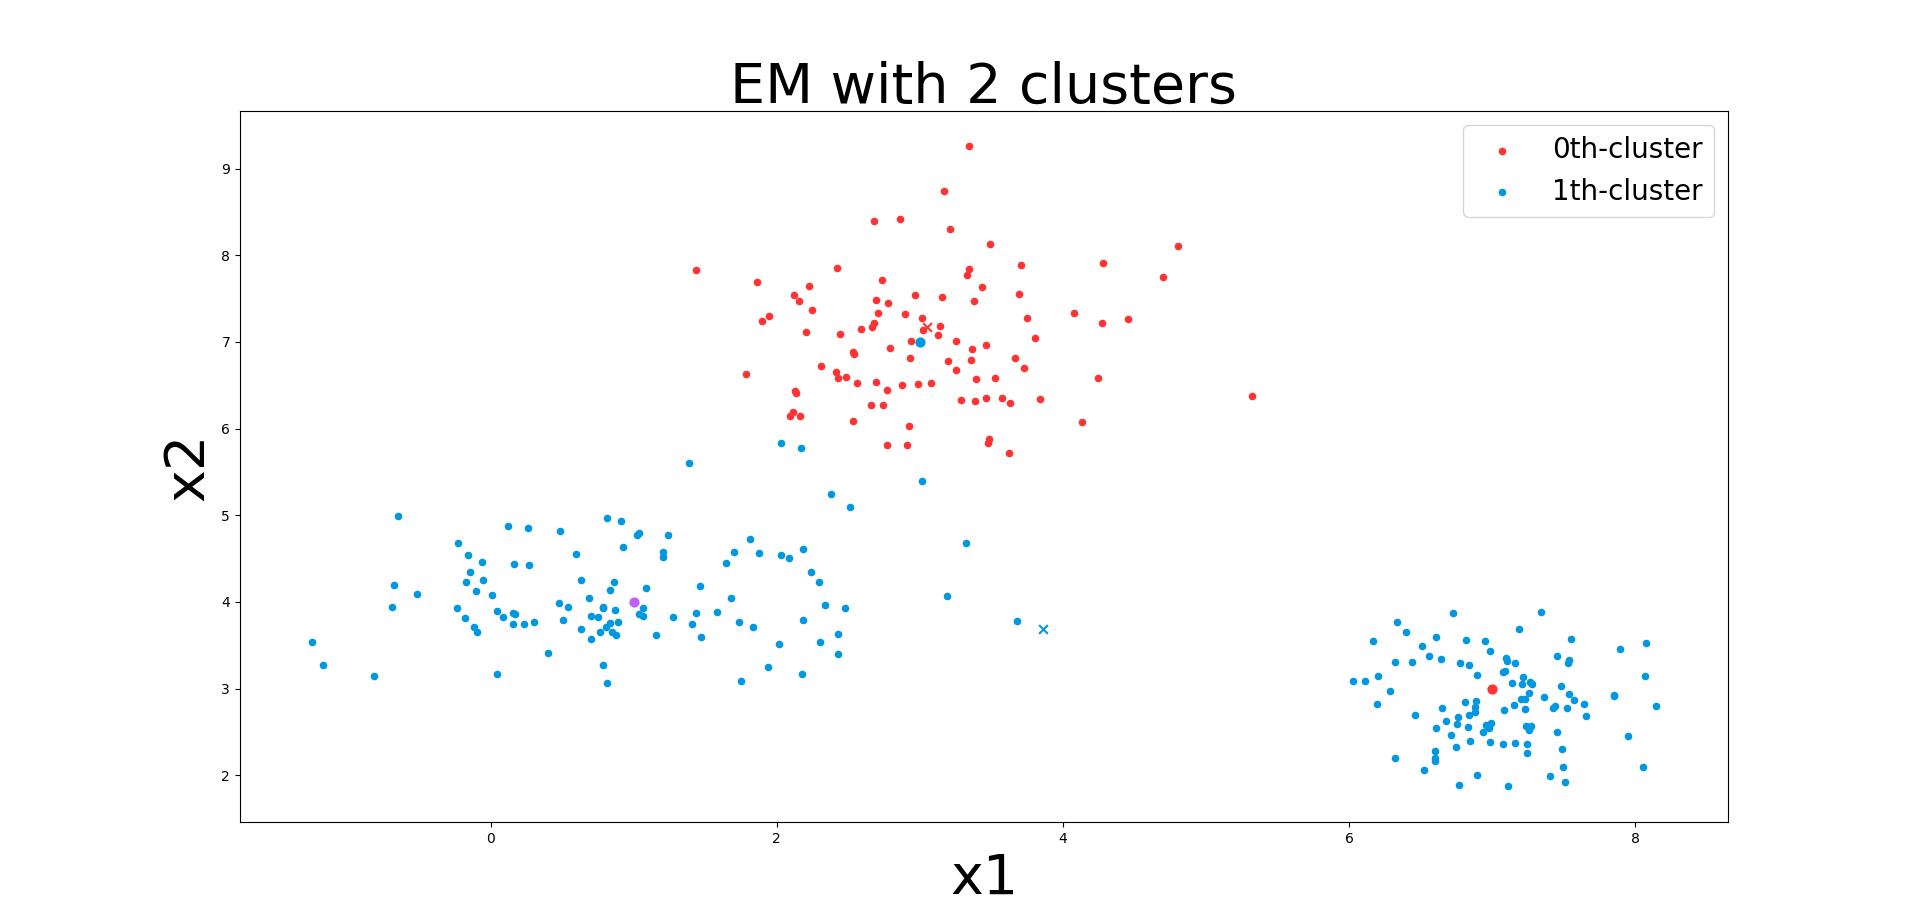
\includegraphics[width=\linewidth, height =3.5cm]{Figs/EM2.png}
			\end{minipage}
			\begin{minipage}[t]{0.25\linewidth}
				\centering	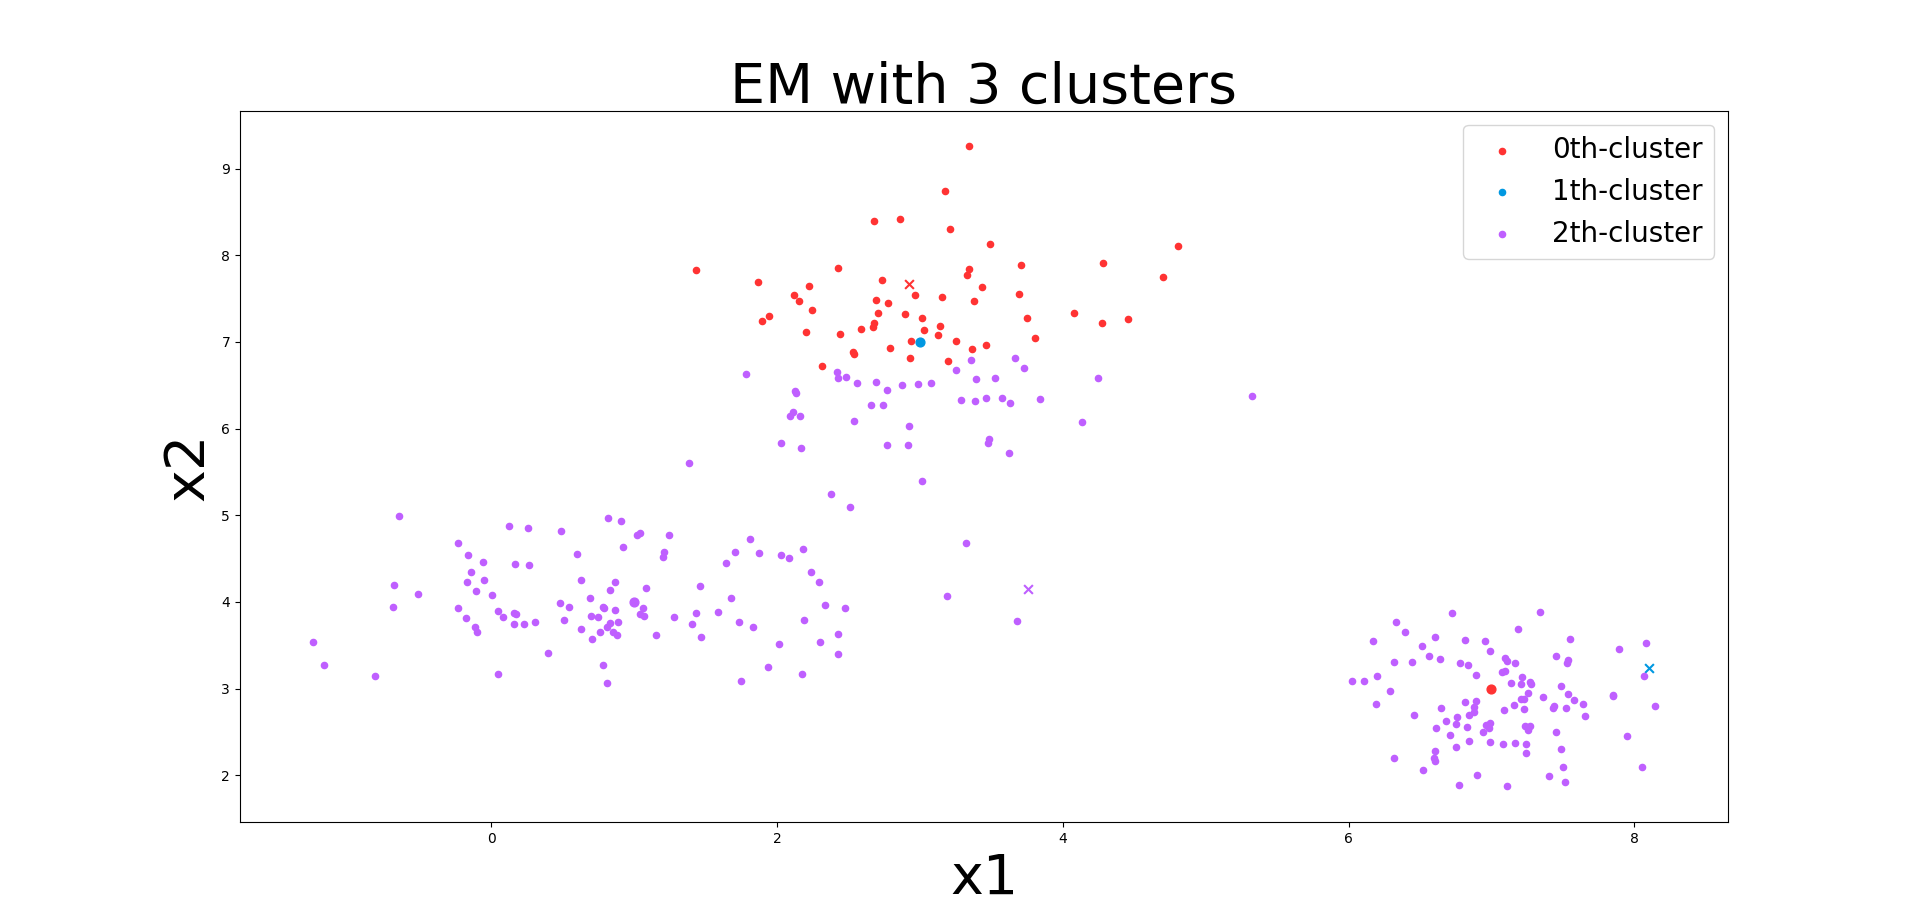
\includegraphics[width=\linewidth, height =3.5cm]{Figs/EM3.png}
			\end{minipage}
			\begin{minipage}[t]{0.25\linewidth}
				\centering	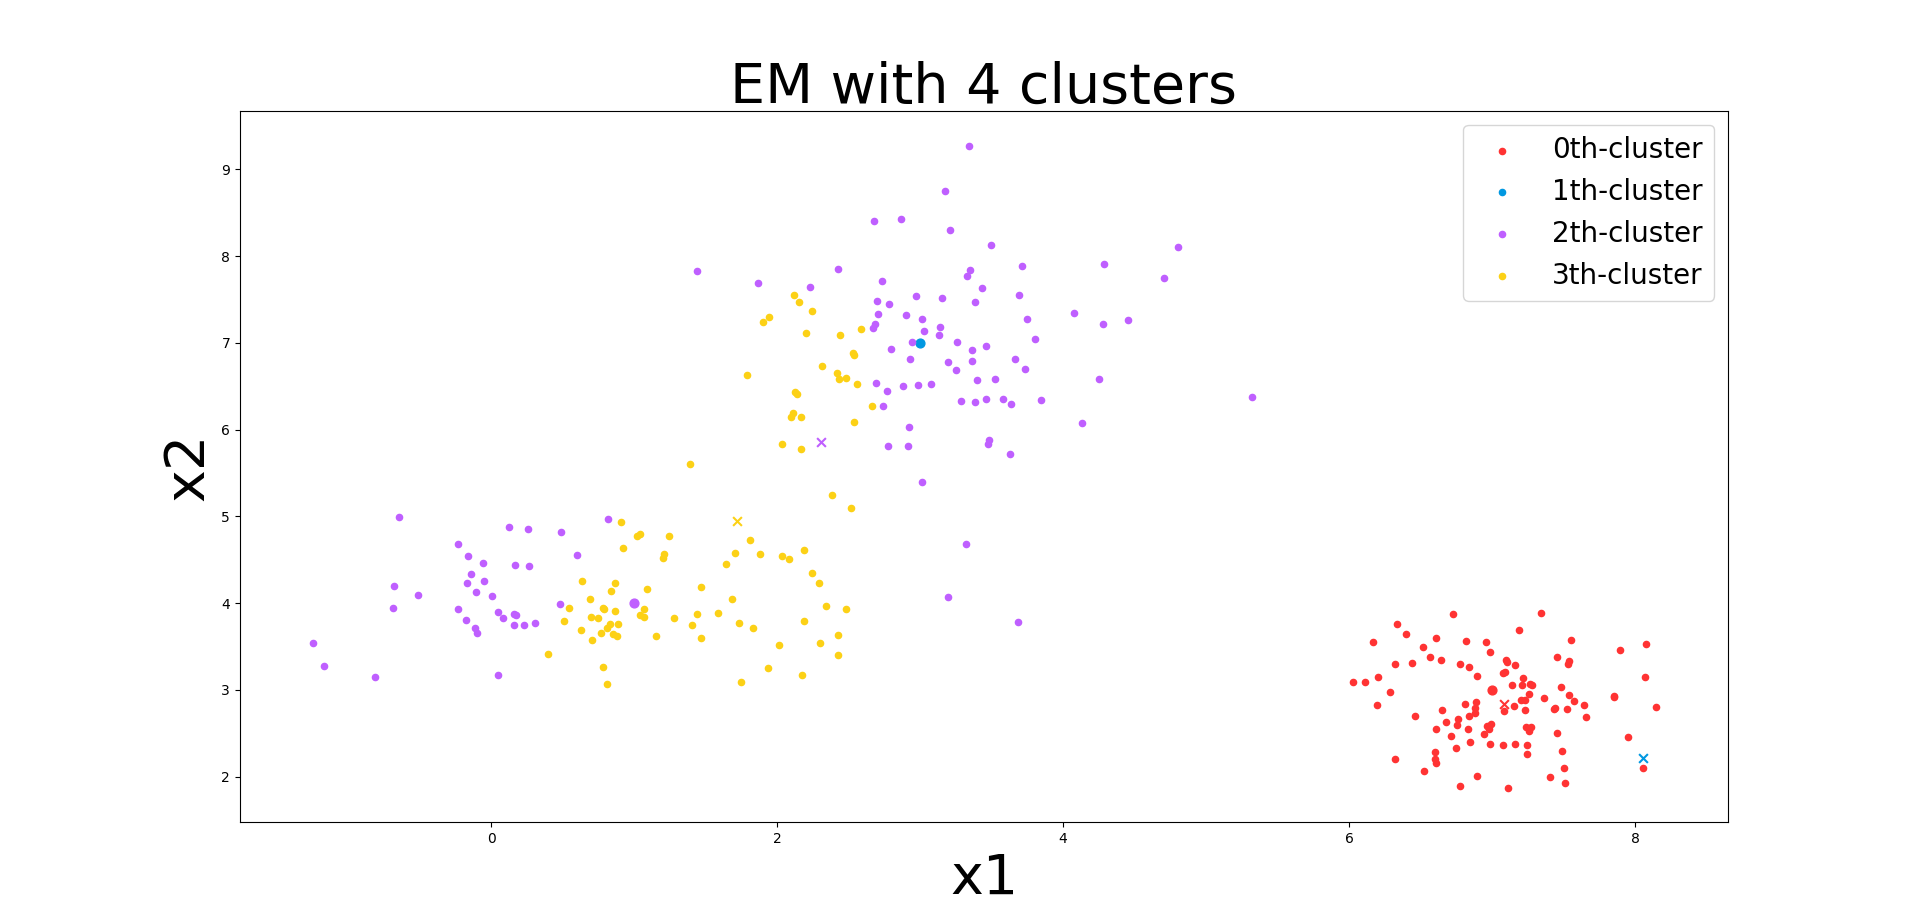
\includegraphics[width=\linewidth, height =3.5cm]{Figs/EM4.png}
			\end{minipage}
			\begin{minipage}[t]{0.25\linewidth}
				\centering	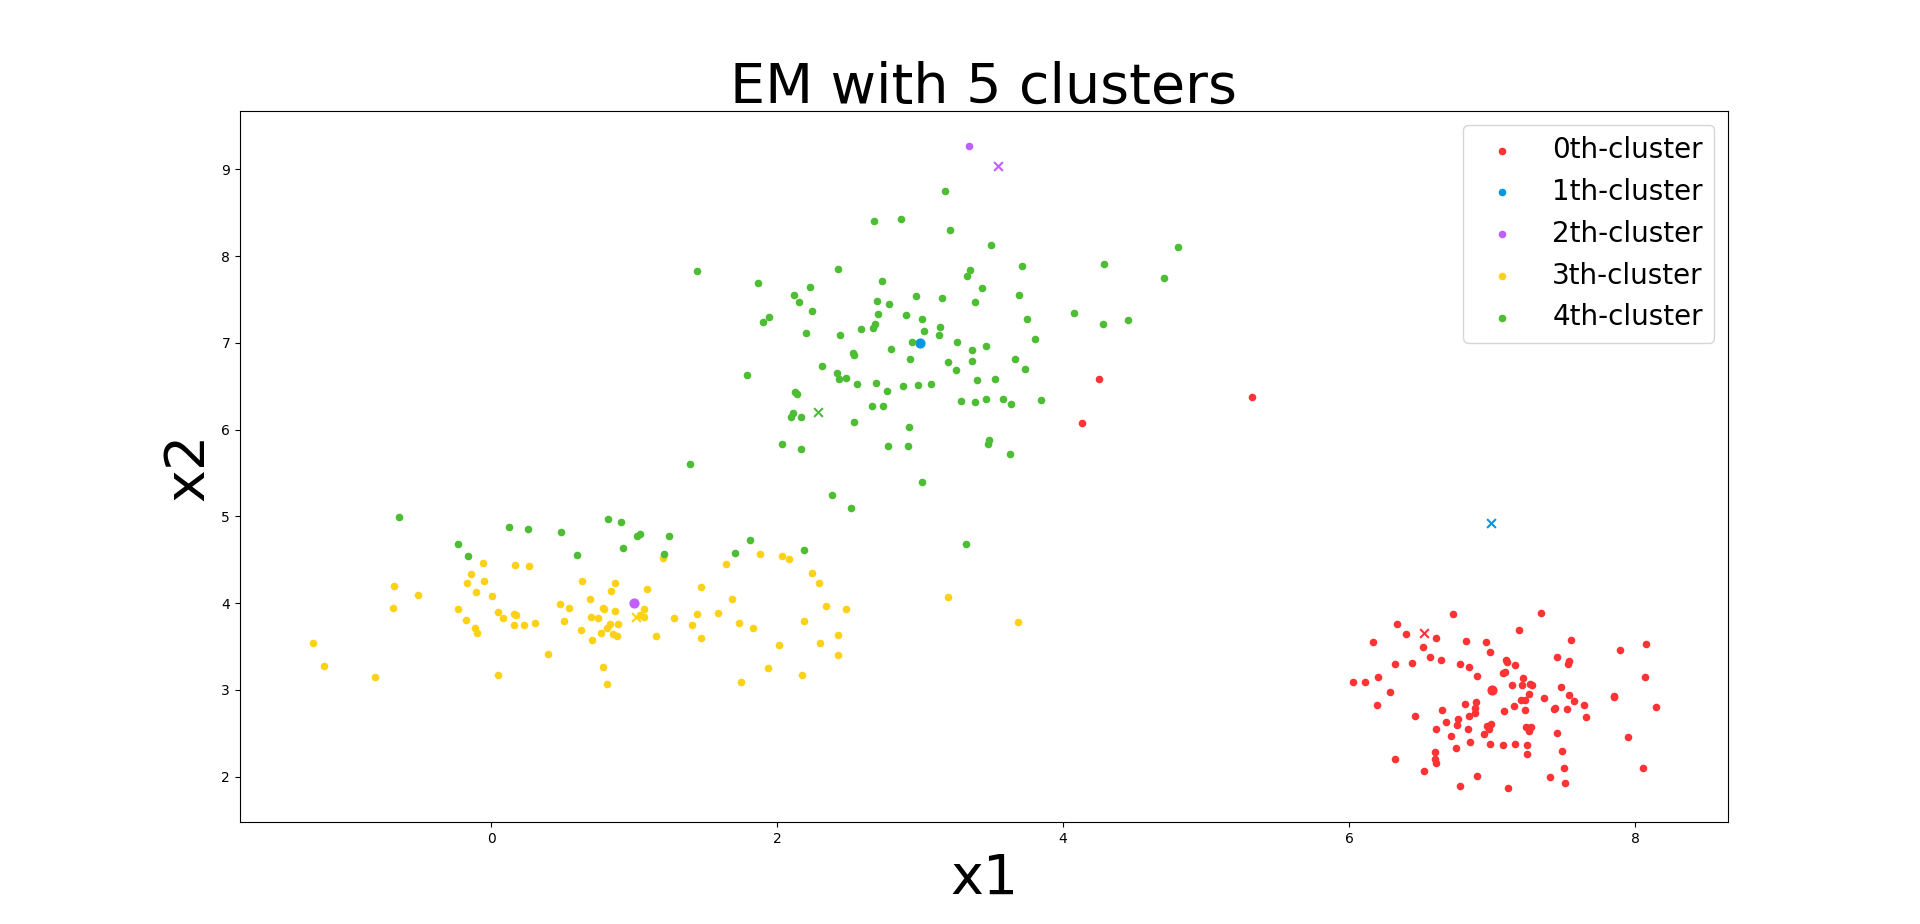
\includegraphics[width=\linewidth, height =3.5cm]{Figs/EM5.png}
			\end{minipage}
		}
		\vspace{-4mm}
		\caption{GMM and EM with different cluster number initialization.}
		\label{fig_GMM_EM}
		\vspace{-4mm}
	\end{figure}

	For VBGMM, we initialize the model with seven clusters, and the result is as Fig. \ref{(fig_VBGMM)} shows. It can be found that VBEM gives a good classification result.
	\begin{figure}[ht]
		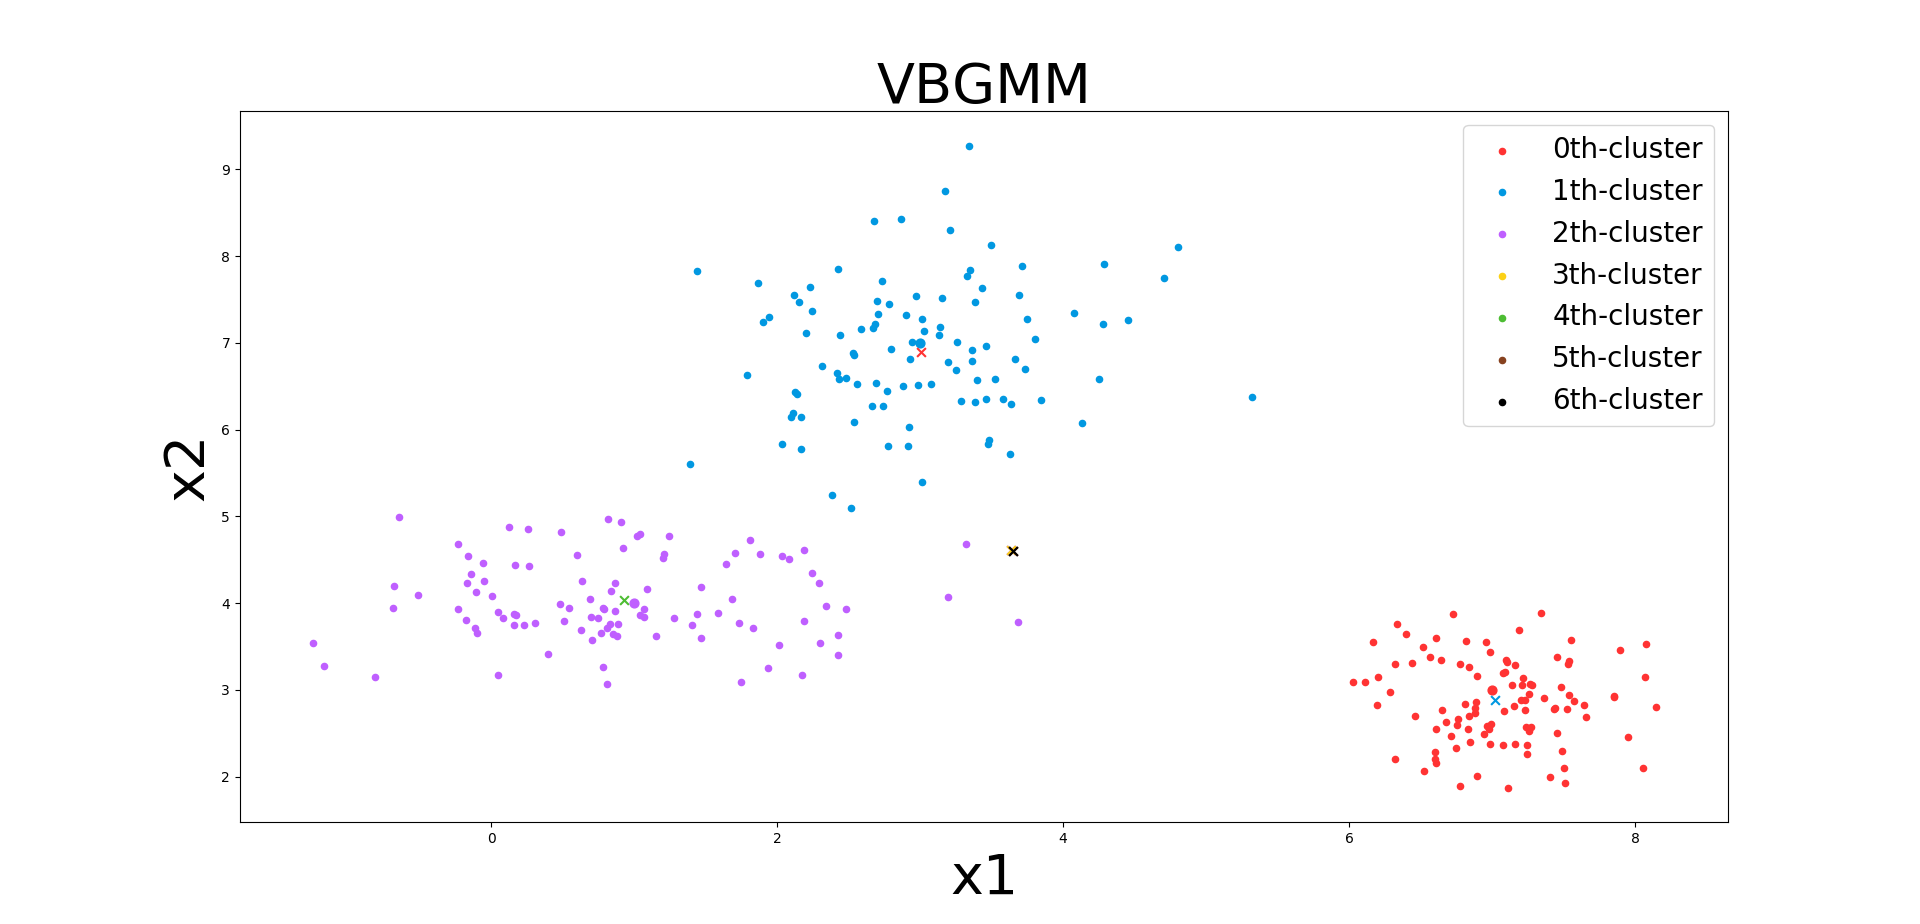
\includegraphics[width=\linewidth]{./Figs/VBGMM.png}
		\caption{VBGMM running result.}
		\label{fig_VBGMM}
	\end{figure}
	
	According to the definition of the AIC and BIC criterion in the slides.
	Akalike's Information Criterion:
	$$\ln p(\Xv_N|\hat{\Theta}_K)-d_k$$
	
	Bayesian Information Criterion:
	$$\ln p(\Xv_N|\hat{\Theta}_K)-\frac{1}{2}d_k\ln N$$


	In the document of the sklearn library, it is said that "The lower the criterion is, the better the model is". In the Fig.~(\ref{fig_criterion}), the upper two sub-figures are derived from GMM model in the sklearn library, and the other two figures are from our EM model. According to the scikit-learn document, we should choose the model with least AIC or BIC score. I change the sign of my AIC function and BIC function to get a positive value. In the upper part of the Fig~(\ref{fig_criterion}), because I initialize the EM algorithm with random cluster position, the AIC and BIC changes every time we run the code. And sometimes they are not helpful in model selection. And if we initialize the EM algorithm with knowledge on the real distribution, the AIC and BIC are nearly the same each time and they are helpful to choose the best model with three cluster. Since the peak of BIC curve is evident than AIC curve, I think BIC is more useful than AIC.
	
	\begin{figure}[ht]
		\centering
		\subfigure[Initialize the clusters with knowledge on real distribution]{
			\centering 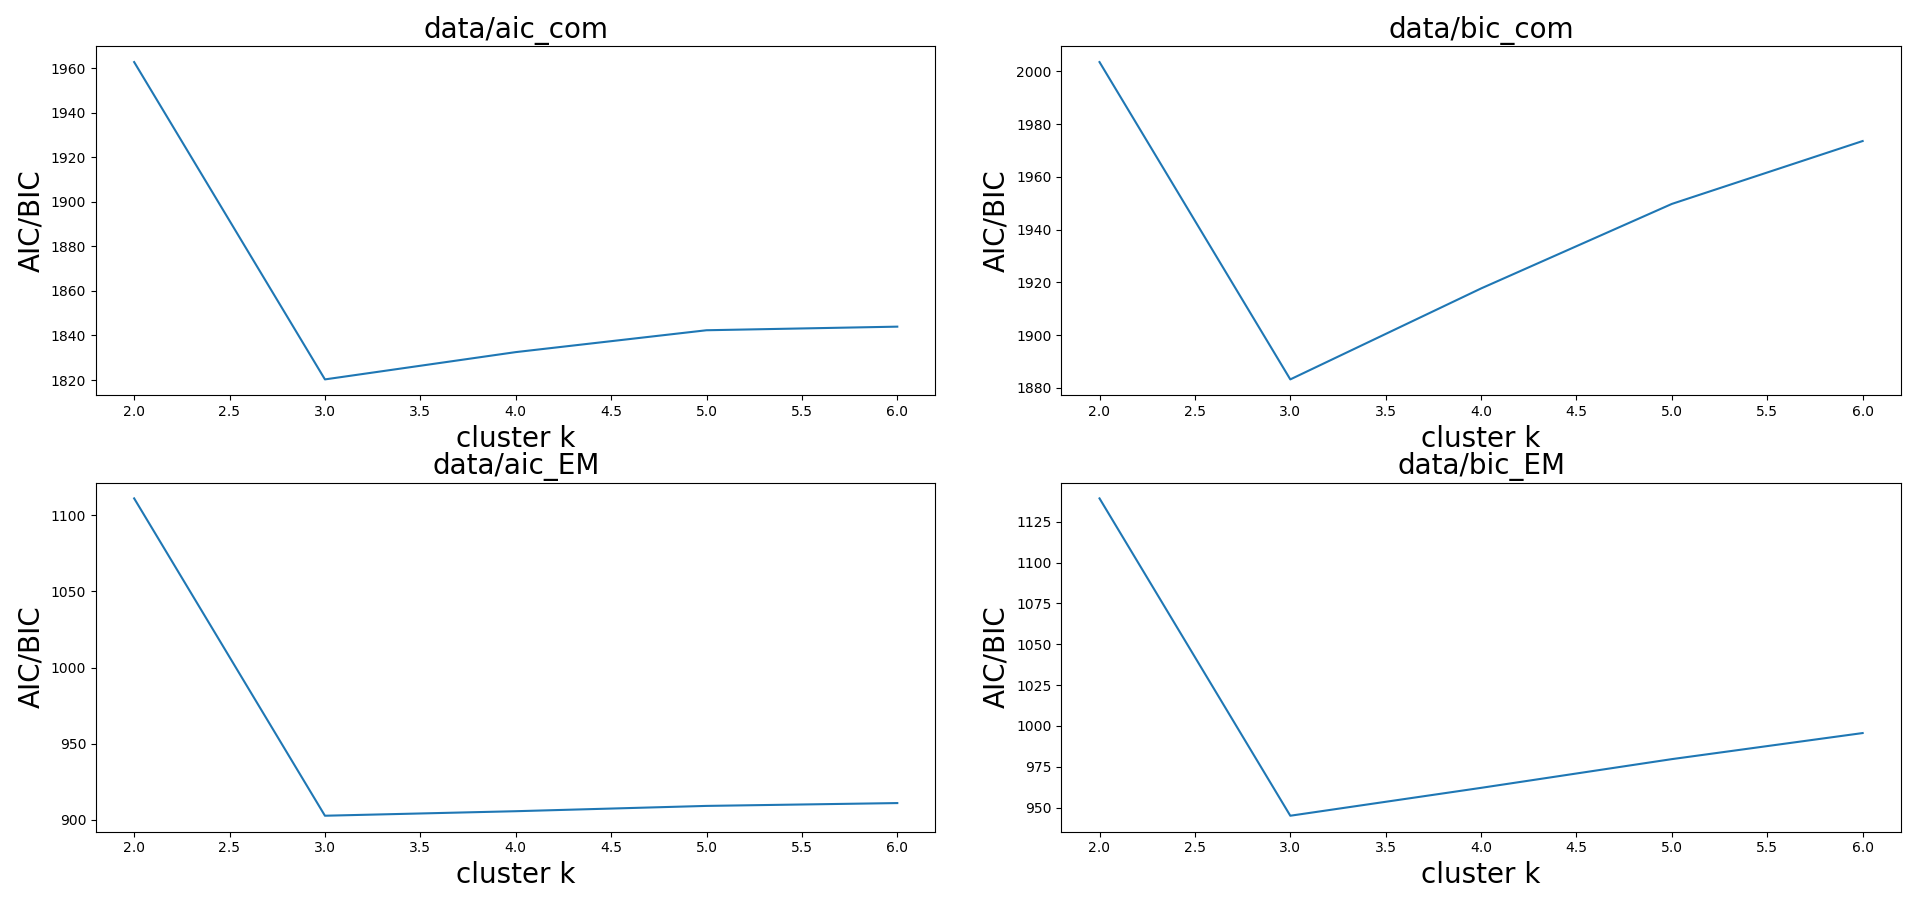
\includegraphics[width=\linewidth]{./Figs/criterion1.png}
		}
		\subfigure[Random initialize the clusters]{
			\centering 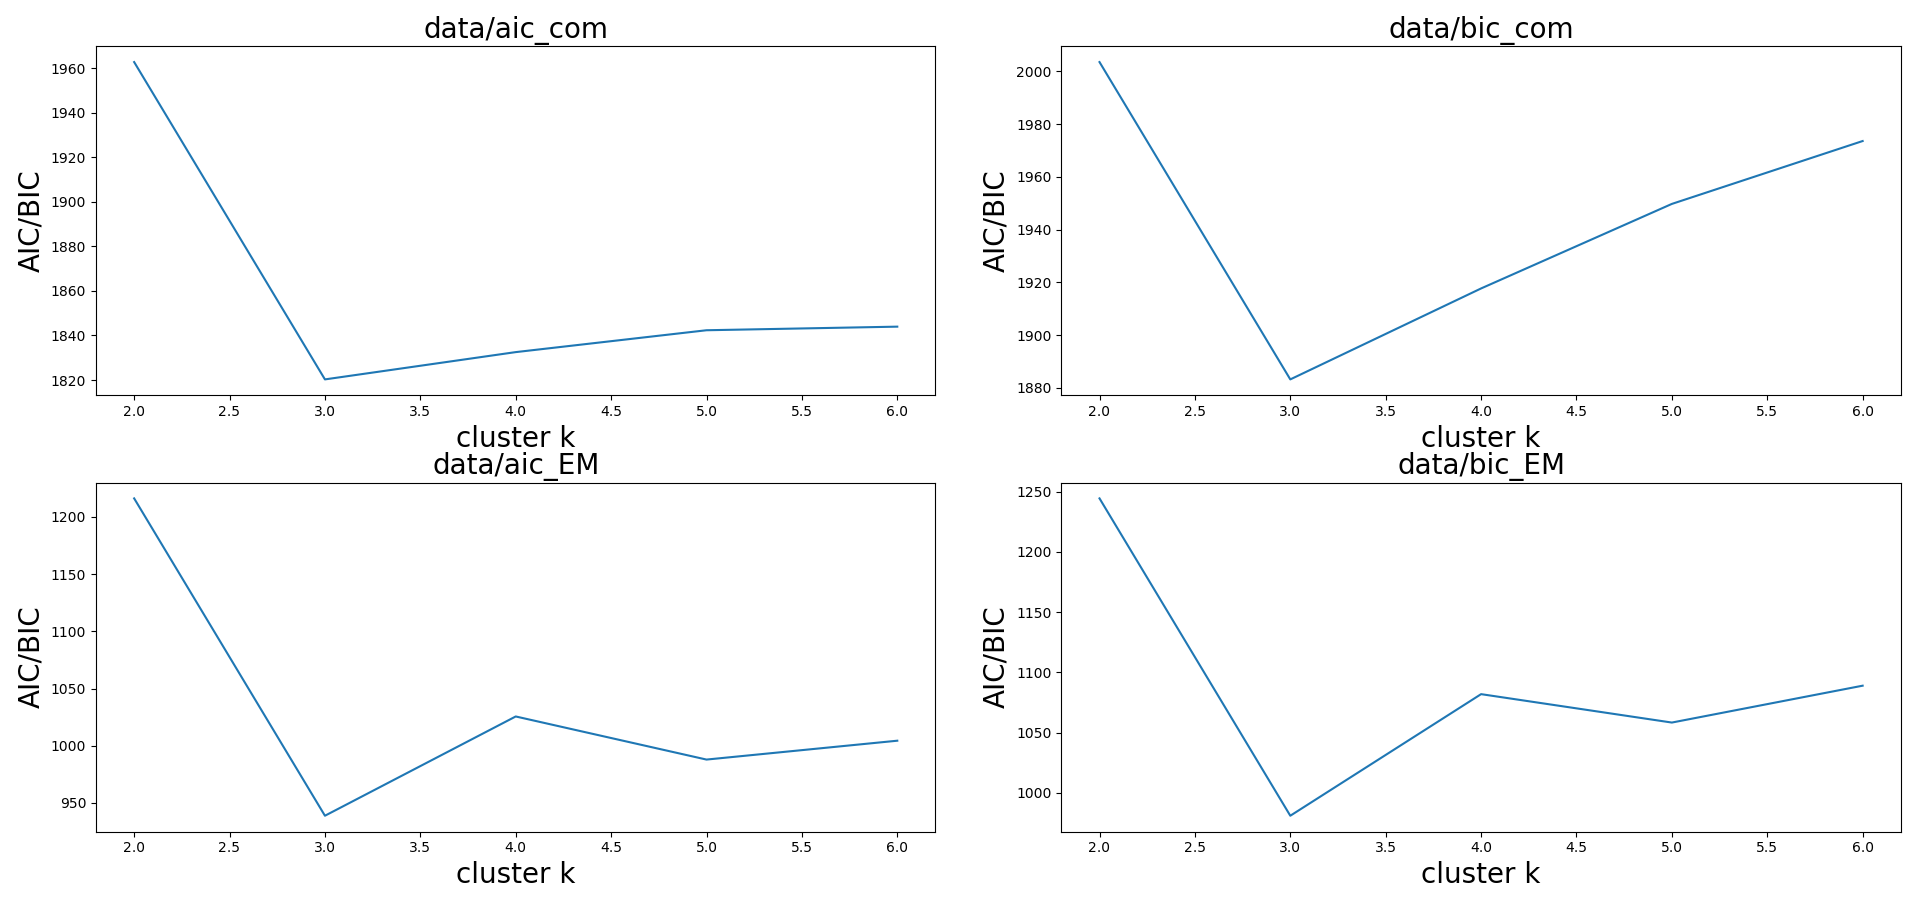
\includegraphics[width=\linewidth]{./Figs/criterion2.png}
		}
		\caption{AIC and BIC criterion of GMM and EM.}
		\label{fig_criterion}
	\end{figure}


	In a word, we can make the conclusion that the models with three clusters are the best models. All of the experiments finally get similar predictions to the real distribution.
\end{sol}

During working on this homework, I learned a lot on the numpy library and sklearn library. Though coding really is tough, it makes me understand the algorithms in the class more thoroughly. The comparison between the famous library and the codes implemented by myself is interesting. Finally, thanks for the help from our teacher and assistants.
\end{hw}

\begin{appendix}
\section{Proposed variant K-mean algorithm}
\begin{breakablealgorithm}
	\caption{Proposed variant K-mean algorithm}
	\label{alg_variant}
	\begin{algorithmic}[1]
		\REQUIRE Prior distribution of $\zv$ (the original $\piv$). Data points $\xv_!,\ldots,\xv_N$.
		\ENSURE The estimated parameters $\muv$ and $\Sigmamat$.
		\STATE Initialize the $\muv_1,\ldots,\muv_K$ and $\Sigmamat_1,\ldots,\Sigmamat_K$.
		\REPEAT
		\FOR{$n \in \{1\to N\}$}
		\STATE $i=0$;
		\STATE $q=0$;
		\FOR{$k\in\{1\to K\}$}
		\STATE $r_{nk}=0$;
		\STATE $p_{nk}=\pi_k\mathcal{N}(\xv_n|\muv_k,\Sigmamat_k)$;
		\IF{$p_{nk}>q$}
		\STATE $q=p_{nk}$;
		\STATE $i=k$;
		\ENDIF
		\ENDFOR
		\STATE $r_{ri}=1$;
		\ENDFOR
		
		\FOR{$k \in \{1\to K\}$}
		\STATE $N_k=0$;
		\FOR{$n\in\{1,\ldots,N\}$}
		\IF{$r_{nk}==1$}
		\STATE $N_k = N_k+1$;
		\ENDIF 
		\ENDFOR 
		\STATE $\pi_k = N_k/N$;
		\STATE $\alphav=\textbf{0}$;
		\FOR{$n\in\{1,\ldots,N\}$}
		\IF{$r_{nk}==1$}
		\STATE $\alphav = \alphav+\xv_n $;
		\ENDIF 
		\ENDFOR
		\STATE $\muv_k = \alpha/N_k$;
		\STATE $\Phimat=\Omat$;
		\FOR{$n\in\{1,\ldots,N\}$}
		\IF{$r_{nk}==1$}
		\STATE $\Phimat = \Phimat+(\xv_n-\muv_k)(\xv_n-\muv_k)^T$;
		\ENDIF 
		\ENDFOR
		\STATE $\Sigmamat_k=\Phimat/N_k$;
		\ENDFOR
		\UNTIL{$\muv~and~\Sigmamat~converge$}
	\end{algorithmic}
\end{breakablealgorithm} 	


\section{Proposed RP K-mean algorithm}
\begin{breakablealgorithm}
	\caption{Proposed RP K-mean algorithm}
	\label{alg_rp}
	\begin{algorithmic}[1]
		\REQUIRE Data points $\xv_!,\ldots,\xv_N$.
		\ENSURE The estimated parameters $\muv$.
		\STATE Initialize the $\muv_1,\ldots,\muv_K$.
		\STATE $t=1$
		\REPEAT
		
		\FOR{$n \in \{1\to N\}$}
		\STATE $i=0$;
		\STATE $j=0$;
		\STATE $q_1=0$;
		\STATE $q_2=0$
		\FOR{$k\in\{1\to K\}$}
		\STATE $r_{nk}=0$;
		\STATE $d_{nk}=$;
		\IF{$p_{nk}>q_1$}
		\STATE $q_1=p_{nk}$;
		\STATE $i=k$;
		\ELSIF{$p_{nk}>q_2$}
		\STATE $q_2=p_{nk}$;
		\STATE $j=k$;
		\ENDIF
		\ENDFOR
		\STATE $r_{ni}=1$;
		\STATE $r_{nj}=-\eta/t$;
		\ENDFOR
		
		\FOR{$k \in \{1\to K\}$}
		\STATE $N_k=0$;
		\FOR{$n\in\{1,\ldots,N\}$}
		\STATE $N_k = N_k+r_{nk}$;
		\ENDFOR
		\STATE $\alphav=\textbf{0}$;
		\FOR{$n\in\{1,\ldots,N\}$}
		\IF{$r_{nk}==1$}
		\STATE $\alphav = \alphav+r_{nk}\xv_n $;
		\ENDIF 
		\ENDFOR
		\STATE $\muv_k = \alphav/N_k$;
		\ENDFOR
		
		\FOR{$j \in \{1\to K\}$}
		\FOR{$k \in \{1\to K\}$}
		\FOR{$n\in\{1,\ldots,N\}$}
		\IF{$r_{nk}<0$}
		\STATE $\muv_j = \muv_j+r_{nk}(\muv_j-\muv_k)$;
		\ENDIF 
		\ENDFOR
		\ENDFOR
		\ENDFOR
		
		\STATE $t=t+1$;
		\UNTIL{$\muv~converge$}
	\end{algorithmic}
\end{breakablealgorithm} 	
\end{appendix}

\end{document}
